% !TEX root = thesis.tex
\section{Open Source Code for Low Resource Languages}
\label{sec:lrl-code}

Now that low resource languages (LRLs) have been described, and now that there has been a brief overview of open source as a software methodology, the reader will doubtless wonder - what is the state of open source code that can be used today by language communities?

Unfortunately, due to the decentralised nature of open source, this is an inherently difficult question to answer. In the ecosystem, there are a few strategies that can be used to inform an answer: use a specific task as a case study for what tools would be used, look at what resources are available from any of the main large data aggregators mentioned in Section~\ref{subsec:resource-aggregators}, take a screenshot of the ecosystem based on some of the more-cited open source tool used for LRL NLP, examine linked open data, and sample relevant work on GitHub through a manually collected list of resources. Each of these strategies is employed in a subsection, below.

\subsection{Case study: Mapping linguistic co\"ordinates}

The breadth of HLT is wide; choosing a specific task within it and then trying to perform that task as adequate as possible would be one way to figure out how much open source code exists, and what that looks like. For example, suppose we were interested in making dialect maps using language co\"ordinates. This is an old research area in linguistics \citep{trudgill1983on,labov2005atlas}, and computational methods for mapping languages have been described in some research, including in the recently started {\it Journal of Linguistic Geography} \citep{labov2012journal}.

For NLP, this is a nontrivial task. Language maps using geolocational data could be used in several ways. For instance, \citep{mccrae2015reconciling} mentions an email sent to the {\it Corpora List} asking for "freely available geotagged tweets collection for research purpose."\footnote{\href{https://mailman.uib.no/public/corpora/2015-February/022044.html}{https://mailman.uib.no/public/corpora/2015-February/022044.html}. \last{April~26}} Geolocation can also be used to plot language relatedness \citep{littauer2012visualizing}.

Another example where geolocation might be useful would be in l10n in the browser. For instance, if the client's browser does not send a {\tt Accept-Language} header\footnote{\href{https://tools.ietf.org/html/rfc7231\#section-5.3.5}{https://tools.ietf.org/html/rfc7231\#section-5.3.5}. \last{April~27}} in their requests to view a website, specifying languages the client understands by using ISO 639 tags,\footnote{\href{https://www.ietf.org/rfc/bcp/bcp47.txt}{https://www.ietf.org/rfc/bcp/bcp47.txt}. \last{April~27}} then the server may use the {\tt Navigator\-Language} object in JavaScript\footnote{\href{https://www.w3.org/TR/html51/webappapis.html\#language-preferences}{https://www.w3.org/TR/html51/webappapis.html\#language-preferences}. \last{April~27}} to query for the language of the browser UI (normally set by the users depending on where they downloaded it), or they could ask the browser directly through the geolocation API (for instance, on Firefox\footnote{\href{https://www.mozilla.org/en-US/firefox/}{https://www.mozilla.org/en-US/firefox/}. \last{April~27}}\footnote{\href{https://developer.mozilla.org/en-US/docs/Web/API/Geolocation/Using_geolocation}{https://developer.mozilla.org/en-US/docs/Web/API/Geolocation/Using\_geolocation}. \last{April~27}}) to supply the geolocation of users and extrapolate plausible languages from this data. Knowing where the user is likely to be, and what languages the user is likely to prefer using, could help with providing their native language automatically in the browser.

\citet{gawne2016mapmaking} give a general overview of the mapping field currently, pointing out that the main resource for finding language geographical co\"ordinates comes from the World Language Mapping System,\footnote{\href{http://www.worldgeodatasets.com/language/.}{http://www.worldgeodatasets.com/language/}. \last{April~25}} a website owned and run by SIL, which are used for ISO 639-3 labelling, and by Glottolog and OLAC. The maps are under a closed license and must be purchased. \citet{gawne2016mapmaking} also mention WALS, which uses its own geographical co\"ordinates, and the ELP, which understandably uses Google Maps as its mapping program, and draws from multiple sources. They also mention Language Landscape,\footnote{\href{http://www.languagelandscape.org/}{http://www.languagelandscape.org}. \last{April~25}} a project which maps instances of language use on a map.

To use these geographic information systems (GIS), one needs to download licensed map data, which could be open or closed. Then, one has to have a mapping software to display that data. This software must also be appropriately licensed. Google Maps is not open source, although it is {\it open access}, in that it is free to use. An open source equivalent of Google Maps is Open Street Maps,\footnote{\href{https://www.openstreetmap.org/}{https://www.openstreetmap.org/}. \last{April~27}} a community built tool that is permissively licensed as CC-BY-SA.\footnote{\href{https://www.openstreetmap.org/copyright}{https://www.openstreetmap.org/copyright}. \last{April~27}} One could use data from Glottolog or the ELP and then map provide a map using Open Street Map while using entirely open source applications, but the end result could be reproduced on Google Maps with the same lack of restrictions - the only difference is that the engine making Google Maps would be a black box.

It is this mixed use case that is most common - researchers or NLP practitioners use a mix of open and closed resources, as needed. \citet{gawne2016mapmaking} mention many programs: Google Earth\footnote{\href{https://www.google.com/earth/}{https://www.google.com/earth/}. \last{April~27}} (closed source, free) for base maps; Geotag\footnote{\href{http://geotag.sourceforge.net/}{http://geotag.sourceforge.net/}. \last{April~27}} (free, open source) and Photo KML\footnote{\href{http://www.visualtravelguide.com/Photo-kml.html}{http://www.visualtravelguide.com/Photo-kml.html}. This URL was provided in \citet{gawne2016mapmaking}, but may be down permanently.} (free) for accessing GIS embedded in pictures taken on iPhones (closed); the KML and KMZ formats,\footnote{\href{http://www.opengeospatial.org/standards/kml/}{http://www.opengeospatial.org/standards/kml/}. \last{April~27}} originally developed by Google for Google Earth but now standards implemented by the Open Geospatial Consortium\footnote{\href{http://www.opengeospatial.org}{http://www.opengeospatial.org}. \last{April~27}} and licensed openly and freely; Koredoko\footnote{\href{https://itunes.apple.com/us/app/koredoko-exif-and-gps-viewer/id286765236}{https://itunes.apple.com/us/app/koredoko-exif-and-gps-viewer/id286765236}. \last{April~27}} for viewing GIS data in photos (closed, free); CartoDB\footnote{\href{https://carto.com/}{https://carto.com/}. \last{April~27}} (proprietary) and CartoCSS\footnote{\href{https://github.com/mapbox/carto}{https://github.com/mapbox/carto}. \last{April~27}} (free, open); TileMill\footnote{\href{https://www.mapbox.com/tilemill/}{https://www.mapbox.com/tilemill/}. \last{April~27}} (free, open, but no longer maintained or updated) and MapBox\footnote{\href{https://www.mapbox.com/mapbox-studio/}{https://www.mapbox.com/mapbox-studio/}. \last{April~27}} (open, freemium) ; QGIS\footnote{\href{https://www.qgis.org/}{https://www.qgis.org/}. \last{April~27}} (free, open); the SQL\footnote{\href{https://www.iso.org/committee/45342/x/catalogue/p/1/u/0/w/0/d/0}{https://www.iso.org/committee/45342/x/catalogue/p/1/u/0/w/0/d/0}. \last{April~27}} language (free, open - languages and formats also have licensing laws and can be copyrighted\footnote{Interestingly, constructed natural languages can also be licensed and copyrighted, leading to legal complications involving corporations suing fan communities for publishing documentation in a given language. Further discussion is out of scope here.}); JPEG\footnote{\href{https://www.iso.org/standard/54989.html}{https://www.iso.org/standard/54989.html}. \last{April~27}} and PNG\footnote{\href{https://www.iso.org/standard/29581.html}{https://www.iso.org/standard/29581.html}. \last{April~27}} image formats (free, open); Adobe PhotoShop\footnote{\href{https://www.adobe.com/products/photoshop.html}{https://www.adobe.com/products/photoshop.html}. \last{April~27}} (closed source, paid); and CartoHexa\footnote{\href{https://www.colorhexa.com/}{https://www.colorhexa.com/}. \last{April~27}} (free, closed).

An example of a mixed workflow would be using a closed source application or website to shim open source data. For example:

\begin{quote}
To give some more general locational context we downloaded some Open Access geopolitical boundaries for Nepal from the Global Administrative Areas website.\footnote{\href{https://gadm.org/download}{https://gadm.org/download}. \last{April~27}} This data was downloaded as KMZ, which TileMill cannot read, so we opened the files in Google Earth (remember ... that KMZ is a compressed KML) and resaved them as KML, which TileMill can read. \citep[228]{gawne2016mapmaking}
\end{quote}

This particular use-case may have benefited from a specific tool which could convert KMZ to KML. A cursory look on GitHub shows 54 repositories that could be relevant,\footnote{\href{https://github.com/search?p=1&q=kmz+kml&type=Repositories}{https://github.com/search?p=1\&q=kmz+kml\&type=Repositories}. \last{April~27}} including one which does solely this task (albeit with Spanish documentation).\footnote{\href{https://github.com/fadamiao/kmz2kml}{https://github.com/fadamiao/kmz2kml}. \last{April~27}} Using an entirely open source pipeline for working with language (or GIS data, as here) is rare, although it is hypothetically possible; however, one quickly runs into problems where open source is concerned, as each subsequent layer of computational processing must then depend upon open source - including the operating system (for instance, GNU/Linux as an open source alternative to the closed Mac OS), processor, silicon chips, and so on. (This is one of the reasons that copyleft remains an issue in licensing.) Idiomatically put: there are turtles all the way down.

As \citet{hu2012multimedia, hu2018web} notes, the general trend in mapping software has been away from native (meaning on the OS level) applications and towards web applications, which may have a steeper learning curve, but which afford remote storage and access, and users over the Internet. WALS uses LeafletJS,\footnote{\href{https://leafletjs.com/}{https://leafletjs.com/}. \last{April~26}} an open source mapping software that uses Open Street Maps as an alternative to using an embedded Google Maps map using their API. \citet{hu2018web} suggests a workflow that uses Leaflet along with jQuery,\footnote{\href{https://jquery.com/}{https://jquery.com/}. \last{April~26}} an open source JavaScript utility library, to display GIS linguistic maps. Web applications can also be used to display geographical data for research; \citet{littauer2013linguistic}, for instance, explored using a SPARQL endpoint to mine RDF data, including geographic location from WALS, to map Dogon languages using Open Street Maps. Further study around using only FLOSS software for displaying GIS data for linguistics is necessary.

\citet{cenerini2017mapping} cite several open source software applications and libraries they used in their study mapping the Cree-Innu-Naskapi continu\"{u}m using data from the Algonquian Linguistic Atlas \citep{junker2011linguistic},\footnote{\href{http://www.atlas-ling.ca/}{http://www.atlas-ling.ca/}. \last{April~26}} but do not open source their own code. This would have been useful, specifically as replicating their study using R \citep{ihaka1996r} would require researchers to write all of their own queries again. More on data privacy will be discussed in Section~\ref{subsec:data-and-privacy}.

This was a small example, looking at only a couple of papers and showing how following open source methodology can be difficult, and how using mixed source applications is often necessary for research and linguistic information. This was a single use case, and every application involving NLP requires navigating software and licensing laws. My purpose in providing this study was to point out how describing the state of open source code that could be used for LRLs is not clear cut. One could argue that this case is reflective of linguistic software, as opposed to NLP or computational linguists. This arbitrary division is not useful, as all actors using language data that has been digitally encoded fall under the wider umbrella of users of human language technology. Languages do not exist within a vacu\"{u}m, and computational linguists using NLP to run deep learning artificial intelligence algorithms on spoken language corpora at scale depend upon previous work done by linguists, language communities, and researchers who spent time on the ground formalising orthographies, compiling dictionaries, and debating the finer points of linguistic minutiae.

That having been said, there are cases where using open source software is decidedly clear cut. For instance, if the goal is to build a part of speech tagger using two hours of annotation, you could use the low-resource-post-tagging-2014 package developed as part of \citet{garrette2013real,garrette2013learning}, and available on GitHub\footnote{\href{https://github.com/dhgarrette/low-resource-pos-tagging-2014}{https://github.com/dhgarrette/low-resource-pos-tagging-2014}. \last{April~27}} without any other considerations than downloading Java and learning a bit of Scala, both free and open source languages. But this is a very limited use case, as this package was built as part of two scientific papers studying this narrowly scoped area.

\subsection{LRL NLP available through data providers}
\label{subsec:lrl-nlp-through-providers}

Rather than exhaustively study each possible use case involving NLP, another strategy is to look at the databases where NLP practitioners, researchers, and language activists find code for their respective languages directly. Using the list of aggregators from Section~\ref{subsec:resource-aggregators}, it is possible to give a general overview of what is available.

The first resource aggregator listed starts on the lower end of the language resource pyramid: Unicode's CLDR resources. Unicode is often the first port-of-call for a language team working on developing scripts for their language, unless the script is already using some  pre\"{e}xisting format (such as the Roman alphabet). CLDR has instructions on checking out their open source subversion repository online.\footnote{\href{http://cldr.unicode.org/index/downloads}{http://cldr.unicode.org/index/downloads}. \last{April~24}} They also have a GitHub repository\footnote{\href{https://github.com/unicode-cldr/cldr-json}{https://github.com/unicode-cldr/cldr-json}. \last{April~24}} and organisation with code for digesting the normally XML representation in JSON, the notation format used most often by JavaScript developers. However, CLDR is not an aggregator - it is more of a suite of tools under one umbrella, as the scope is limited to working with the Unicode format.

Finding resources is not easy. The Endangered Languages Project, for instance, contains information on over 3000 languages, and catalogues 6830.\footnote{\href{http://www.endangeredlanguages.com/resources/}{http://www.endangeredlanguages.com/resources/}. \last{April~24}} None of these resources are code: the searchable formats are: Format, Image, Video, Document, Audio, Link, Guide. Glottolog only has academic references, and ODIN only has interlinear glossed text (IGT) corpora. Omniglot describes alphabets but does not index tooling for them. CLARIN has thousands of resources - but none of them are code, and you need to be an accredited researcher from a European institution to access them. The ELRA site provides hundreds of corpora resources - for purchase. The LRE Map\footnote{\href{http://www.resourcebook.eu/searchll.php}{http://www.resourcebook.eu/searchll.php}. \last{April~27}} is incredibly useful, in that it has around two thousand resources which are searchable; however, there are no links provided to any resource, and the accessibility or licensing of these resources is not listed. The language search functionality is currently not functioning, and the data is not machine accessible.\footnote{As of April~27, 2018.}

The Linguistic Data Consortium has a tool page,\footnote{\href{https://www.ldc.upenn.edu/language-resources/tools}{https://www.ldc.upenn.edu/language-resources/tools}. \last{April~26}} where it notes five tools that may be useful for researchers using its data. These tools are Annotation Graph Kit (AGTK), The Champollion Toolkit, the LDC Word Aligner, Sphere Conversion tools, and XTrans, of which only Sphere has a non-standard license that allows use but may have more restrictions. This suite of tools is particularly useful for dealing with LDC data. This sort of tool and corpus bundling is common; when building a resource, the tools to manage that resource are included directly in a tools page. DoBes has the same type of page,\footnote{\href{http://dobes.mpi.nl/archive_info/tools/}{http://dobes.mpi.nl/archive\_info/tools/}. \last{April~26}} where they mention tools developed at The Language Archive: ELAN,\footnote{\href{https://tla.mpi.nl/tools/tla-tools/elan/}{https://tla.mpi.nl/tools/tla-tools/elan/}. \last{April~26}} a powerful tool for time aligned annotation of video or audio data; ARBIL, a metadata catalogue creation tool; LAMUS, a tool for uploading data and metadata into the DoBes archive and for managing existing collections; and LEXUS, a web-based lexicon tool. This scale is common, but there are some archives that have more tools listed. For instance, the Resource Network for Linguistic Diversity (RNLD), a largely Australian network, lists dozens of tools and applications that could be useful.\footnote{\href{http://www.rnld.org/software}{http://www.rnld.org/software}. \last{April~26}} The list does not differentiate between bundled code that works as an application on the OS, and code which must be downloaded and run through a terminal. EMELD, the Electronic Metastructure for Endangered Languages Data (a short-term project run through LDC, the ELF, and the Universities of Arizona, Eastern Michigan, and Wayne State) has a similar list with hundreds of items.\footnote{\href{http://emeld.org/school/toolroom/software/software-display.cfm}{http://emeld.org/school/toolroom/software/software-display.cfm}. \last{April~26}}

For field linguistics, this mixture of apps and small tooling is common, as is combining corpora with tools in some fashion. For instance, \citet{caballero2017choguita} presents a fieldwork paper on Choguita Rar�muri (Tarahumara), an Uto-Aztecan language. In the paper, they mention using Microsoft Word\footnote{\href{https://products.office.com/en-CA/word}{https://products.office.com/en-CA/word}. \last{April~26}} and Excel,\footnote{\href{https://products.office.com/en-CA/excel}{https://products.office.com/en-CA/excel}. \last{April~26}} SIL's Fieldwork Language Explorer (FLEx),\footnote{\href{http://software.sil.org/fieldworks/download/.}{http://software.sil.org/fieldworks/download/}. \last{April~26}} and show screenshots of Quicktime.\footnote{\href{https://support.apple.com/quicktime}{https://support.apple.com/quicktime}. \last{April~26}} The corpus they present is stored on the Endangered Language Archive at SOAS, University of London\footnote{\href{elar.soas.ac.uk/deposit/0056}{elar.soas.ac.uk/deposit/0056}. \last{April~26}} \citep{caballero2009data}. The majority of these tools are closed source, except for FLEx. However, they also mention using ELAN. \citet{caballero2017choguita} made their own tools to work with ELAN, and they made this code available on GitHub.\footnote{\href{https://github.com/ucsd-field-lab/kwaras}{https://github.com/ucsd-field-lab/kwaras}. \last{April~26}} In order to access the data, the reader is likely to have read the paper; thus the document, the code, and the corpus together form a unit of research, which are all used together.

OLAC, with hundreds of thousands of resources, has a tooling page,\footnote{\href{http://www.language-archives.org/tools.html}{http://www.language-archives.org/tools.html}. \last{April~26}} which mainly helps with working with OLAC as opposed to pointing to resources which can be used with language data. Unfortunately, searching for software resources comes up short. A short look at a specific language, Nask\-api, shows 23 resources,\footnote{\href{http://www.language-archives.org/language/nsk}{http://www.language-archives.org/language/nsk}. \last{April~26}} most of which are published papers - except for the Cr\'ubad\'an archive, the Glottolog reference, typological references on WALS and on the Rosetta Project, and a pointer to resources noted on the LINGUIST List, which lists no resources when accessed.\footnote{\href{https://linguistlist.org/olac/search-olac.cfm?LANG=nsk}{https://linguistlist.org/olac/search-olac.cfm?LANG=nsk}. \last{April~26}} Scottish Gaelic is not much different (26 resources),\footnote{\href{http://www.language-archives.org/language/gla}{http://www.language-archives.org/language/gla}. \last{April~26}} although it does point to some corpora.

META-SHARE, which aggressively pursues open access and open licensing for resources in its database, has 344 tools available, and allows easy searching for these tools,\footnote{\href{http://www.meta-share.org/}{http://www.meta-share.org}. \last{April~26}} although signing up as a user is necessary. The ACL Wiki has resources for 84 languages.\footnote{\href{https://aclweb.org/aclwiki/List_of_resources_by_language}{https://aclweb.org/aclwiki/List\_of\_resources\_by\_language}. \last{April~26}} From a random selection of these resources (including corpora), one could get an idea of how many resources are totally aggregated: Arabic (16), Navajo (1), Catalan (8), Faroese (4), Galician (20), Maltese (4), Irish (10). LT-World lists 523 separate tools (this number was reached by adding up all resource amounts listed on their language tools page\footnote{\href{http://www.lt-world.org/kb/resources-and-tools/language-tools/}{http://www.lt-world.org/kb/resources-and-tools/language-tools}. \last{April~26}} and assuming that there is no duplication of tools, which may be inaccurate). These tools are for all languages, and only a subset could be understood to apply to LRLs.

These collected resources are, to my knowledge, the main place to look for aggregated data around software resources on particular languages. This overview was brief; more fine-tuned exploration of the numbers of packages would likely not improve our understanding of the ecosystem. From this, it is clear that there are global open source software resources in the order of hundreds, not thousands. Considering that thousands of languages have not ascended digitally, this is neither unexpected nor ideal.

\subsection{Linked open data}
\label{subsec:lod}

The aggregators mentioned in Section~\ref{subsec:lrl-nlp-through-providers} are largely massive databases which store corpora on their own servers, or were HTML pages that linked directly to other resources using hardcoded links. OLAC is an exception; it uses an XML representation of the Dublin Core metadata set \citep{dublin1998dublin}, and uses infrastructure based on the Open Archives Initiative.\footnote{\href{http://www.openarchives.org}{http://www.openarchives.org}. \last{April~26}} OLAC uses a protocol on top of this to pool resources from many sources; resources which wish to be entered need to have metadata which conforms to a certain standard, and then they can be aggregated \citep{simons2001olac}. The CLARIN VLO \citep{mccrae2015one} also use the OAI-PMH protocol \citep{sompel2004resource, mccrae2015reconciling}. These two providers - among others - do not pull from each other naturally.

Linghub and the Linguistics Linked Data cloud were both created to resolve these issues. The latter is a linked data ontology created by the Open Linguistics Working Group (OWLG) \citep{chiarcos2011working, chiarcos2012open, chiarcos2013building, mccrae2016open}, largely by manually selecting linguistic data sources from Datahub.io for aggregation. The Linguistic Linked Open Data (LLOD) cloud \citep{chiarcos2012linking} can be previewed at \href{http://linguistic-lod.org}{\nolinkurl{http://linguistic-lod.org}},\footnote{\href{http://linguistic-lod.org/}{http://linguistic-lod.org}. \last{April~26}} and in Figure~\ref{fig:llod}.

\begin{figure}
 \centering
 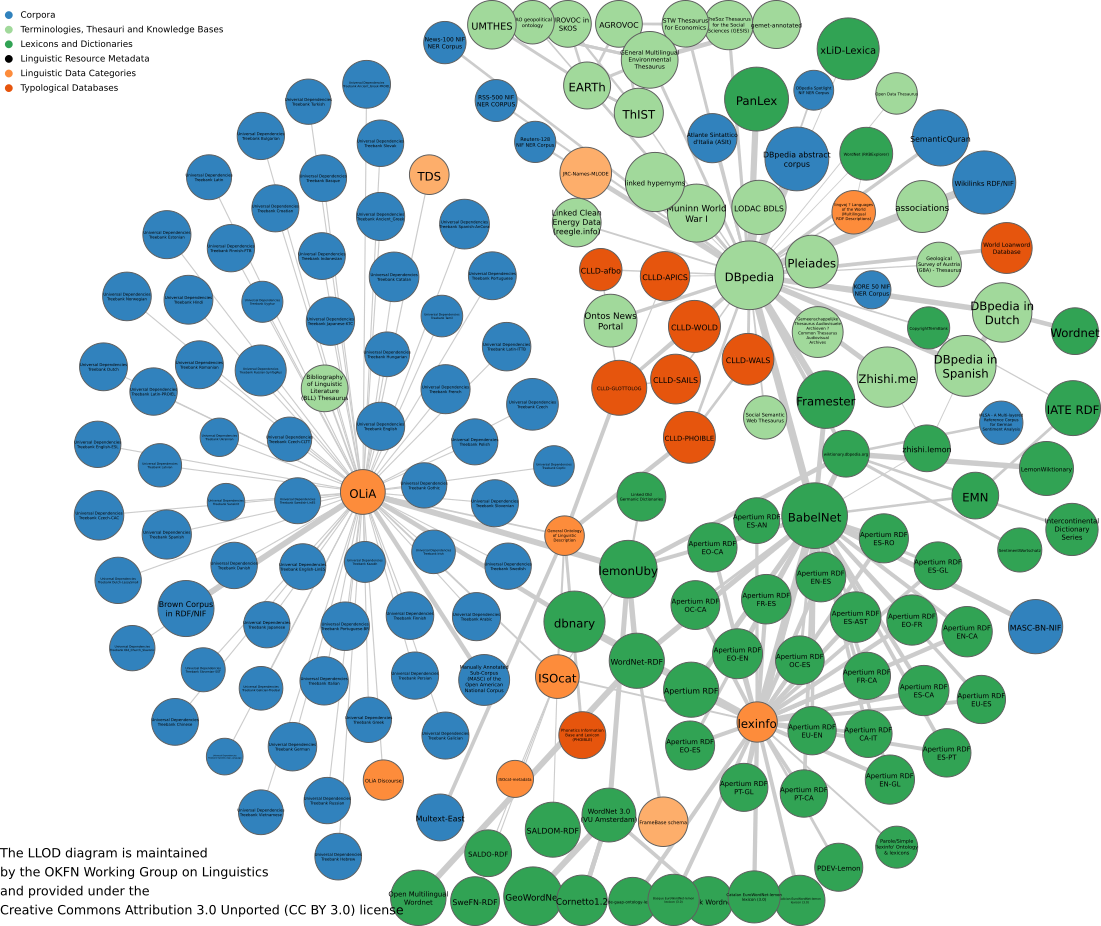
\includegraphics[width=1\textwidth]{img/llod.png}
 \caption{The Linguists Linked Open Data cloud \citep{chiarcos2012linking}}
 \label{fig:llod}
\end{figure}

Linghub \citep{mccrae2015linghub, mccrae2015reconciling} was created to allow for mining of all available databases - including META-SHARE, LRE Map, Datahub, and CLARIN's VLO - using SPARQL, a query language that works for Semantic Web ontologies encoded in RDF. Since publishing \citet{mccrae2015linghub}, OLAC has allowed its resources to also be mined.\footnote{\href{http://www.language-archives.org/news.html\#llod}{http://www.language-archives.org/news.html\#llod}. \last{April~26}} At this point, there are few large repositories of language resource data which are unable to be queried. However, linked data has the existential failing of only including metadata which has been included in the available data sources. It is a fantastic resource for finding corpora, and \citet{mccrae2015linghub} gives several examples of finding data through the cloud;  it is also an exceptional way to mine the LRE map database, which provides names of language resources for NLP tooling. But there is a barrier to entry of learning SPARQL and using an available portal, and any work outside of the curated, largely academic resources may not be available.

The linked open data cloud and Linghub also do not explicitly cater to LRLs, although there has been some work in this area \citep{huang2017linking}.

\subsection{Multilingual NLP libraries}
\label{subsec:popular-open-source-libraries}

While searching for code that has been tagged with metadata noting the language it serves has some merits, there are also possibilities for using generic code on many languages. For instance, \citet{bender2016linguistic} explores the field of multilingual NLP (now decades old; for instance, \citet{kay1997proper} called for this in the 90s), pointing out that there is a growing body of research that uses language typology to abstract and identify language features which allow for applying NLP systems from one language to another.

\begin{quote}
Businesses developing commercial products with NLP are interested in the markets represented by {\tt low resource languages} (LRLs; i.e., those languages for which there are not many digitized data sets or basic NLP systems such as part-of-speech taggers or morphological or syntactic parsers), some of which represent very large populations in emerging economies. Finally, researchers looking to apply NLP techniques to assist in LRL documentation are naturally interested in developing NLP systems that work across very diverse languages.\citep[646]{bender2016linguistic}
\end{quote}

\citet{bender2016linguistic} goes on to mention the LinGo Matrix system \citep{bender2002grammar, drellishak2005coordination} that can be used to create rule-based grammars for natural languages using linguistic typographical data. The LinGo Matrix, and all work within the DELPH-IN system (a collaboration looking mainly at the Head-Driven Phrase Structure Grammar and Minimal Recursion Semantics) is open source.\footnote{\href{http://www.delph-in.net/wiki/index.php/Software}{http://www.delph-in.net/wiki/index.php/Software}. \last{April~26}}

They also mention projecting resources across languages, such as \citet{yarowsky2001inducing}, who projected linguistic annotations like POS tags and noun phrase parsing from English to French and Chinese, by using bilingual texts that had been word-aligned. This was extended in the previously mentioned \citet{agic2015if}, who similar POS tagger projection for one hundred LRLs. Their code is open source on Bitbucket.\footnote{\href{https://bitbucket.org/lowlands/}{https://bitbucket.org/lowlands/}. \last{April~26}}

This avenue of research is fascinating and broad, because it allows for small tools to be applied to other LRLs at a minimal cost. A study involving looking at all of the available research, with an in-depth look in each scientific article that includes links to source code, would be warranted and welcomed. It is unfortunately largely out of scope for this thesis; it is enough, here, to know that open source code for LRLs is dependent upon academics working in this field sharing their code on large repositories, and that this code must also be adapted to each particular LRL, which, while an extensive task, is made easier through multilingual NLP and cross-linguistic projection.

At a lower level, there are NLP toolkits which are useful for working with LRL datasets, which are language agnostic. The most well known is arguably the Natural Language Toolkit (NTLK)\footnote{\href{http://www.nltk.org/}{http://www.nltk.org/}. \last{April~26}} \citep{bird2006nltk}, a free and open source Python library that enables users to interface with over fifty different corpora and lexical resources, and which provides a suite of tools such as tokenizers and parsers which can be used in sparse data contexts. A primer written by the main creators \citep{bird2009natural}\footnote{Available online at \href{http://nltk.org/book}{http://nltk.org/book}. \last{April~26}} is used frequently in natural language processing classes written by the creators. It is licensed under the Apache 2.0 license, an open source license. \footnote{\href{https://github.com/nltk/nltk/blob/develop/LICENSE.txt}{https://github.com/nltk/nltk/blob/develop/LICENSE.txt}. \last{April~26}} On GitHub, there are currently 204 contributors listed,\footnote{\href{https://github.com/nltk/nltk/graphs/contributors}{https://github.com/nltk/nltk/graphs/contributors}. \last{April~10}} and the contribution history in Git shows 234 (found by using the command {\tt git authors}). Some of the resources within NLTK work especially well with LRLs. For instance, in 2015, NLTK added machine translation libraries, including popular ones such as IBM Models 1-3 and BLEU.

By open sourcing their code, the NLTK authors have allowed it to be adapted and re-used. Currently, there are several ports, or reimplementations in another programming language which allows use in different coding language ecosystems. One of these is the JavaScript language implementation.\footnote{\href{https://github.com/NaturalNode/natural}{https://github.com/NaturalNode/natural}. \last{April~26}} This has 6700 stars on GitHub, which, since they reflect favouritism from individual users, is a good indicator of community vitality and use, and 88 contributors. The port is also open source, under an MIT license.\footnote{\href{https://github.com/NaturalNode/natural\#license}{https://github.com/NaturalNode/natural\#license}. \last{April~26}}

It is difficult to track usage of these open source software packages by LRL communities or researchers, as, once downloaded, there are no convenient metrics which lead back to the original source. Code, when run, generally leaves no trace. Again, the fundamental problem of tracking LRL open source software inhibits understanding the ecosystem, but it is clear from individual anecdotes and through scientific citations that work is being done in this area.

\subsection{A GitHub database for open source code}
\label{sec:solutions}

\begin{quote}
Currently, two approaches to metadata collection for language resources can be distinguished. Firstly, we distinguish a curatorial approach to metadata collection in which a repository of language resource metadata is maintained by a cross-institution organization ... This approach is characterized though high-quality metadata that are entered by experts, at the expense of coverage. A collaborative approach, on the other hand, allows anyone to publish language resource metadata. ... A process for controlling the quality of metadata entered is typically lacking for such collaborative repositories, leading to less qualitative metadata and inhomogeneous metadata resulting from free-text fields, user-provided tags and the lack of controlled vocabularies.
\end{quote}

\citet{mccrae2015linghub}, above, note that there are multiple ways of collecting metadata around resources, which provide their motivation to combine the two in Linghub. Here, I present a database built using a combination of the two; a curatorial, crowd-sourced database of language resources. This database has a mild advantage over Linghub and other large databases in that it is also decentralised, easily accessible and readable without learning a new language, and has a lower barrier to data entry.

Presented first in \citet{CCURL}, {\tt low-resource-languages} is a list of code resources for LRLs available on GitHub, available (under my namespace) at \href{https://github.com/RichardLitt/low-resource-languages}{https://github.com/RichardLitt/low-resource-languages}.\footnote{This was formerly called {\tt endangered-languages}. It was renamed to reflect attitudes mentioned in Section~\ref{subsubsec:response}.} The list is structured in Markdown,\footnote{\href{https://daringfireball.net/projects/markdown/syntax}{https://daringfireball.net/projects/markdown/syntax}. \last{April~26}} a lightweight format for text that is rendered natively on GitHub and is an industry standard in open source for structuring text documents.

Instead of using an XML or RDF representation that needs to be shown through a portal, this list natively works as a text list, as well, although the metadata is not as well structured and does not lend itself to aggregation in the same fashion. Making a scraper that would automatically translate the data into XML would be trivial. However, the benefit of using Markdown is that anyone on GitHub can easily parse and analyse the data directly, and that anyone can access and submit patches to add to the list. On GitHub, social coding conventions surrounding patches - called {\it pull requests} - allows for easy quality assurance of the data, as anyone suggesting an addition or deletion has to wait for a code maintainer to verify that their contribution is up to standard. This allows for a curated, collaborative approach to documentation and metadata aggregation. Curation occurs largely through my acceptance of related pull requests, along with other maintainers of the list - currently, Hugh Patterson of SIL,\footnote{\href{https://github.com/HughP}{https://github.com/HughP}. \last{April~26}} @cesine\footnote{\href{https://github.com/cesine}{https://github.com/cesine}. \last{April~26}} and @AnnaLuisaD of the Living Tongues Institute.\footnote{\href{https://github.com/AnnaLuisaD}{https://github.com/AnnaLuisaD}. \last{April~26}}

To date, there are 19 authors as recorded through {\tt git authors}, and 17 contributors recorded through GitHub's contributor view.\footnote{\href{https://github.com/RichardLitt/low-resource-languages/graphs/contributors}{https://github.com/RichardLitt/low-resource-languages/graphs/contributors}. \last{April~26}} Most pull requests came from @cesine, followed by @HughP. Six users contributed more than two pull requests. This data\footnote{\href{https://gist.github.com/RichardLitt/e60bcf9f399939b16181bf25ad6da8ba}{Available at https://gist.github.com/RichardLitt/e60bcf9f399939b16181bf25ad6da8ba}. \last{April~26}} came from an analysis of contributions using the GitHub API by using the {\tt name-your-contributors}\footnote{\href{https://github.com/mntnr/name-your-contributors/}{https://github.com/mntnr/name-your-contributors/}. \last{April~27}} tool, by running {\tt name-your-contributors -u RichardLitt -r low-resource-languages}.

A large majority of these files were last touched by me,\footnote{This figure was calculated by running {\tt git blame README.md | grep "Richard" | wc -l}.} as I have frequently reorganised and edited the list. In the past two weeks, GitHub's traffic shows 217 views by 37 unique visitors.\footnote{\href{https://github.com/RichardLitt/low-resource-languages/graphs/traffic}{https://github.com/RichardLitt/low-resource-languages/graphs/traffic}. \last{April~26}} There are a total of 39 forks, which reflects users who have copied the code to their own namespace (necessary for suggesting changes back to the main {\tt master} branch in GitHub). There are 166 stars and 24 watchers as of this writing.

There are 441 links available in the list,\footnote{This figure was calculated by running \texttt{grep "\textbackslash* \textbackslash[" README.md | wc -l}.} with hundreds of general resources and 32 different subsections available for specific low resource languages. Instead of tagging resources directly, they are placed in single sections that best describe the resource. The language specific sections are for: Albanian, Alutiiq, Amharic, Arabic, Bengali, Chichewa, Galician, Georgian, Guarani, Hausa, Hindi, H\o gnorsk, Inuktitut, Irish, Kinyarwanda, Lingala, Lushootseed, Malay, Malagasy, Manx, Migmaq, Minderico, Nishnaabe, Oromo, Quechua, Sami, Scottish Gaelic, Secwepemcts\'in, Somali, Tigrinya, Yiddish, and Zulu. Other sections cover: Single language lexicography projects and utilities, Utilities, Software, Keyboard Layout Configuration Helpers, Annotation, Format Specifications, i18n-related Repositories, Audio automation, Text-to-Speech
Text automation, Experimentation, Flashcards, Natural language generation, Computing systems, Android Applications, Chrome Extensions, FieldDB, FieldDB Webservices / Components / Plugins, Academic Research Paper Specific Repositories, Example Repositories, Language \& Code Interfaces, Fonts, Corpora, Organizations On GitHub, Other OSS Organizations, and Tutorials.

An example entry is provided below, for {\tt fast\_align} \citep{dyer2013simple}. The syntax of the example is as follows: A bullet point to place the item in a list; A link within brackets pointing to the GitHub repository where the open source code is stored, or to the resource elsewhere; and a basic description taken from the repository.

\begin{quote}
{\tt * [fast\_align](https://github.com/clab/fast\_align) - Simple, fast unsupervised word aligner.}
\end{quote}

In \citet{CCURL}, we described how the list is aimed at project managers, community developers doing language development, linguists, and software developers, mentioning some cases where developers reached out to say thank you for the list. To summarise our description: the list is for everyone, and the ease of accessibility of GitHub and rendered Markdown make it suitable for any audience. We did not then highlight how being on GitHub is of paramount importance. It is GitHub's social platform, and their extensive community, which makes this list most relevant. Since most open source code is on GitHub, then it follows that facilitating discovery by putting metadata directly on the site is useful step to undertake. As well, since the code is in an open source, Git repository, it is entirely possible for someone to easily copy the list and continue development and curation if for any reason my own copy goes down for any reason.

At LREC 2016 in Portoro\v{z}, where \citet{CCURL} was presented during the poster session\footnote{In reality, I presented it from my laptop as a way of facilitating input and discussion, as I felt that the analog quality of a poster would not properly convey the usefulness of the list, and as it was difficult to physically source a poster while hitchhiking from Italy.}, I collected responses on a Google Form from attendees (similar to data sourcing for LRE Maps, in some ways). There were 18 respondents. All but one of them said they have code related to LRLs; only six of them had GitHub accounts (although one more had a Bitbucket account). Some of them have since contributed to the list.

There were at least two complaints; one of list quality, and another that the pages and subpages are often dead. The second concern has been fixed by implementing {\tt awesome\_bot},\footnote{\href{https://github.com/dkhamsing/awesome_bot}{https://github.com/dkhamsing/awesome\_bot}. \last{April~26}} a tool which automatically checks all of the links and ensures that they resolve, and continuous integration tests with it through TravisCI.\footnote{\href{https://travis-ci.org/RichardLitt/low-resource-languages}{https://travis-ci.org/RichardLitt/low-resource-languages}. \last{April~26}} I have also cloned all of the Sourceforge repositories into GitHub repositories, to ensure that the open source licensed code is available in the GitHub ecosystem.

There is ongoing work to do curating the list, gathering sources, and improving the sections where data is stored. And, in the end, the magnitude of software resources is similar to what is found on any of the larger aggregators. It is unfortunately impossible to judge click-throughs and downloads of the list beyond what is provided above, given the nature of GitHub repositories and software. However, many tools mentioned in this list are not available on other providers - some novelty as an aggregator can be assumed. As \citet{CCURL} has no citations on Google Scholar as of yet, I assume that marketing work for the list is another future need to be met.

\subsection{Data and privacy}
\label{subsec:data-and-privacy}

Above, I have endeavoured to show that the state of open source work for LRLs is difficult to determine. Neither curated resources, linked aggregators of all resources, or mining the scientific literature are able to sufficiently answer the questions of how much code is out there, of what quality is that code, and where can language resource consumers best find their tools. However, it is probable that researchers working on a given language could easily find references to code which is relevant to their language, if it exists, using one of these three methodologies.

Unfortunately, a large amount of both data and tooling over that data is still not permissively licensed or available. Historically, linguists have not permissively licensed or provided open access to their corpora; it is specifically to combat this that large frameworks like the LDC or META-SHARE were created. However, these organisations do not solve some of the underlying issues regarding sharing data.

One issue which is unresolved is that of aligning incentives for researchers to open their research. Researching takes time and funding; opening up research to others can be seen as an act of na\"{i}ve altruism, especially in cases where the work could be easily used by competitive labs or businesses. For corpora to be open, providers may need to feel that they will be properly remunerated for the work. For some, this is less of a worry than citations and prestige. Citing linguistic data is not the same as citing research papers in journals or conferences, and only recently have there been movements towards citing data in itself. For instance, the Austin Principles for Data \citep{AustinPrinciples2017} were recently created to set guidelines for citing linguistic data. It emphasises that data is important and legitimate in the research cycle, that credit and attribution are needed where due, that it should be provided as evidence whenever there is a claim, that it should be referred to with DOIs that are persistent and unique, that it should be openly accessible, that it should be verifiable and specific to claims made, as well as interoperable and flexible in format. Each of these points could be expanded; for instance, evidentiality implies that in certain situations, producers should open confidential information if they wish to make a claim academically; for instance, Google researchers publishing results from their MT systems must also make their corpora available.

These principles can be extended to software, which historically is not cited academically (as in this paper, where a footnote to a website has for the most part sufficed). There is ongoing work in the sciences (if not in linguistics directly) on enforcing software citations \citep{DBLP:journals/corr/KatzCWHVHSJCCVL15, katz2016report}. The previously mentioned {\it Journal of Open Source Software} \citep{smith2018journal} is a good example of an effort to make code a citable object. To my knowledge, there has been no major effort linking linguistics corpora and the related tools under the same citable object. More research and collaboration here would be welcome.

Another facet regarding sharing data revolves around the sensitive nature of linguistic data itself, and ethical issues surrounding researchers or corpus architects. Participants who initially provide linguistic data may require permanent access to that data, and may wish to restrict access to others - for instance, in the case where stories or data are viewed as part of their cultural heritage, and which they view as private to their culture. Linguists taking data need to then document the wishes of the participants; and convey this on to data providers, to ensure that archivists respect the participants and the linguists wishes. Data which is gathered electronically {\it en masse} can  also lead to difficulties, as not all participants wishes can be easily taken into account (for instance, with large databases made by web crawlers). This milieu of needs and obligations can lead to licensing and access complications, especially with regard to LRLs. For instance, Chiarcos raised a question on the Open Linguistics mailing list\footnote{\href{https://lists.okfn.org/mailman/listinfo/open-linguistics}{https://lists.okfn.org/mailman/listinfo/open-linguistics}. \last{April~27}} regarding the legality of sharing Bible translations under EU and US law, and whether or not reuse of this data would constitute copyright violations for researchers who use the data.\footnote{\href{https://lists.okfn.org/pipermail/open-linguistics/2017-April/001359.html}{https://lists.okfn.org/pipermail/open-linguistics/2017-April/001359.html}. \last{April~27}} (There was no clear resolution in this case). There is a host of active research and discussion around this topic; \citet{liberman2000legal, newman2007copyright, rice2006ethical, austin2010communities, o2010ethical, cushman2013wampum} are recommended for further reading.

Sometimes, privacy revolves less around the users or the language communities, and more around researchers not wishing to open source their code until they are done developing their project, or until a grant ends, or until they are safe that they wo not be scooped by other researchers. Other factors include the brevity of some academic funding cycles, concerns about scope, or lack of education regarding how open source works. However, the landscape is changing slowly. For instance, in a paper describing a tool for sharing interlinearised and lexical data in different formats, \citet[132]{kaufman2018kratylos} note that "Kratylos will be made open-source and accessible to the public through a GitHub repository at the end of the current grant period. Kratylos is built entirely from open- source software itself and transcodes proprietary media formats into the open-source codecs Ogg Vorbis (for audio) and Ogg Theora (for video)."\footnote{To date, this has not been open sourced. \href{http://elalliance.org/programs/documentation/kratylos/}{\nolinkurl{http://elalliance.org/programs/documentation/kratylos/}}. \last{April~27}} This is particularly insightful, as it shows that open source archives can arise out of initial closed-source development. Open source is not always a static state for code; and it is becoming more common to see open source code for LRL NLP as researchers become more familiar with current trends in software development.

% Removed as we cover this, basically, in Open Source
%\subsection{Data permanence and interoperability}

%\subsubsection{i18n documentation for larger open source tools}
%In some cases, tools themselves may canonically be used for NLP, but may also be translated into LRLs, thus allowing LRL developers to use the code themselves for bootstrapping their tools. For example, Node has an i18n and l10n committee that works to translate tools - and there is some interested in working with LRLs. % This may be a stretch.
%Another instance would be code which has been ported into rare languages % cite uspanteko work in java
